


% Header, overrides base

    % Make sure that the sphinx doc style knows who it inherits from.
    \def\sphinxdocclass{article}

    % Declare the document class
    \documentclass[letterpaper,10pt,english]{/Library/Python/2.7/site-packages/sphinx/texinputs/sphinxhowto}

    % Imports
    \usepackage[utf8]{inputenc}
    \DeclareUnicodeCharacter{00A0}{\\nobreakspace}
    \usepackage[T1]{fontenc}
    \usepackage{babel}
    \usepackage{times}
    \usepackage{import}
    \usepackage[Bjarne]{/Library/Python/2.7/site-packages/sphinx/texinputs/fncychap}
    \usepackage{longtable}
    \usepackage{/Library/Python/2.7/site-packages/sphinx/texinputs/sphinx}
    \usepackage{multirow}

    \usepackage{amsmath}
    \usepackage{amssymb}
    \usepackage{ucs}
    \usepackage{enumerate}

    % Used to make the Input/Output rules follow around the contents.
    \usepackage{needspace}

    % Pygments requirements
    \usepackage{fancyvrb}
    \usepackage{color}
    % ansi colors additions
    \definecolor{darkgreen}{rgb}{.12,.54,.11}
    \definecolor{lightgray}{gray}{.95}
    \definecolor{brown}{rgb}{0.54,0.27,0.07}
    \definecolor{purple}{rgb}{0.5,0.0,0.5}
    \definecolor{darkgray}{gray}{0.25}
    \definecolor{lightred}{rgb}{1.0,0.39,0.28}
    \definecolor{lightgreen}{rgb}{0.48,0.99,0.0}
    \definecolor{lightblue}{rgb}{0.53,0.81,0.92}
    \definecolor{lightpurple}{rgb}{0.87,0.63,0.87}
    \definecolor{lightcyan}{rgb}{0.5,1.0,0.83}

    % Needed to box output/input
    \usepackage{tikz}
        \usetikzlibrary{calc,arrows,shadows}
    \usepackage[framemethod=tikz]{mdframed}

    \usepackage{alltt}

    % Used to load and display graphics
    \usepackage{graphicx}
    \graphicspath{ {figs/} }
    \usepackage[Export]{adjustbox} % To resize

    % used so that images for notebooks which have spaces in the name can still be included
    \usepackage{grffile}


    % For formatting output while also word wrapping.
    \usepackage{listings}
    \lstset{breaklines=true}
    \lstset{basicstyle=\small\ttfamily}
    \def\smaller{\fontsize{9.5pt}{9.5pt}\selectfont}

    %Pygments definitions
    
\makeatletter
\def\PY@reset{\let\PY@it=\relax \let\PY@bf=\relax%
    \let\PY@ul=\relax \let\PY@tc=\relax%
    \let\PY@bc=\relax \let\PY@ff=\relax}
\def\PY@tok#1{\csname PY@tok@#1\endcsname}
\def\PY@toks#1+{\ifx\relax#1\empty\else%
    \PY@tok{#1}\expandafter\PY@toks\fi}
\def\PY@do#1{\PY@bc{\PY@tc{\PY@ul{%
    \PY@it{\PY@bf{\PY@ff{#1}}}}}}}
\def\PY#1#2{\PY@reset\PY@toks#1+\relax+\PY@do{#2}}

\expandafter\def\csname PY@tok@gd\endcsname{\def\PY@tc##1{\textcolor[rgb]{0.63,0.00,0.00}{##1}}}
\expandafter\def\csname PY@tok@gu\endcsname{\let\PY@bf=\textbf\def\PY@tc##1{\textcolor[rgb]{0.50,0.00,0.50}{##1}}}
\expandafter\def\csname PY@tok@gt\endcsname{\def\PY@tc##1{\textcolor[rgb]{0.00,0.27,0.87}{##1}}}
\expandafter\def\csname PY@tok@gs\endcsname{\let\PY@bf=\textbf}
\expandafter\def\csname PY@tok@gr\endcsname{\def\PY@tc##1{\textcolor[rgb]{1.00,0.00,0.00}{##1}}}
\expandafter\def\csname PY@tok@cm\endcsname{\let\PY@it=\textit\def\PY@tc##1{\textcolor[rgb]{0.25,0.50,0.50}{##1}}}
\expandafter\def\csname PY@tok@vg\endcsname{\def\PY@tc##1{\textcolor[rgb]{0.10,0.09,0.49}{##1}}}
\expandafter\def\csname PY@tok@m\endcsname{\def\PY@tc##1{\textcolor[rgb]{0.40,0.40,0.40}{##1}}}
\expandafter\def\csname PY@tok@mh\endcsname{\def\PY@tc##1{\textcolor[rgb]{0.40,0.40,0.40}{##1}}}
\expandafter\def\csname PY@tok@go\endcsname{\def\PY@tc##1{\textcolor[rgb]{0.53,0.53,0.53}{##1}}}
\expandafter\def\csname PY@tok@ge\endcsname{\let\PY@it=\textit}
\expandafter\def\csname PY@tok@vc\endcsname{\def\PY@tc##1{\textcolor[rgb]{0.10,0.09,0.49}{##1}}}
\expandafter\def\csname PY@tok@il\endcsname{\def\PY@tc##1{\textcolor[rgb]{0.40,0.40,0.40}{##1}}}
\expandafter\def\csname PY@tok@cs\endcsname{\let\PY@it=\textit\def\PY@tc##1{\textcolor[rgb]{0.25,0.50,0.50}{##1}}}
\expandafter\def\csname PY@tok@cp\endcsname{\def\PY@tc##1{\textcolor[rgb]{0.74,0.48,0.00}{##1}}}
\expandafter\def\csname PY@tok@gi\endcsname{\def\PY@tc##1{\textcolor[rgb]{0.00,0.63,0.00}{##1}}}
\expandafter\def\csname PY@tok@gh\endcsname{\let\PY@bf=\textbf\def\PY@tc##1{\textcolor[rgb]{0.00,0.00,0.50}{##1}}}
\expandafter\def\csname PY@tok@ni\endcsname{\let\PY@bf=\textbf\def\PY@tc##1{\textcolor[rgb]{0.60,0.60,0.60}{##1}}}
\expandafter\def\csname PY@tok@nl\endcsname{\def\PY@tc##1{\textcolor[rgb]{0.63,0.63,0.00}{##1}}}
\expandafter\def\csname PY@tok@nn\endcsname{\let\PY@bf=\textbf\def\PY@tc##1{\textcolor[rgb]{0.00,0.00,1.00}{##1}}}
\expandafter\def\csname PY@tok@no\endcsname{\def\PY@tc##1{\textcolor[rgb]{0.53,0.00,0.00}{##1}}}
\expandafter\def\csname PY@tok@na\endcsname{\def\PY@tc##1{\textcolor[rgb]{0.49,0.56,0.16}{##1}}}
\expandafter\def\csname PY@tok@nb\endcsname{\def\PY@tc##1{\textcolor[rgb]{0.00,0.50,0.00}{##1}}}
\expandafter\def\csname PY@tok@nc\endcsname{\let\PY@bf=\textbf\def\PY@tc##1{\textcolor[rgb]{0.00,0.00,1.00}{##1}}}
\expandafter\def\csname PY@tok@nd\endcsname{\def\PY@tc##1{\textcolor[rgb]{0.67,0.13,1.00}{##1}}}
\expandafter\def\csname PY@tok@ne\endcsname{\let\PY@bf=\textbf\def\PY@tc##1{\textcolor[rgb]{0.82,0.25,0.23}{##1}}}
\expandafter\def\csname PY@tok@nf\endcsname{\def\PY@tc##1{\textcolor[rgb]{0.00,0.00,1.00}{##1}}}
\expandafter\def\csname PY@tok@si\endcsname{\let\PY@bf=\textbf\def\PY@tc##1{\textcolor[rgb]{0.73,0.40,0.53}{##1}}}
\expandafter\def\csname PY@tok@s2\endcsname{\def\PY@tc##1{\textcolor[rgb]{0.73,0.13,0.13}{##1}}}
\expandafter\def\csname PY@tok@vi\endcsname{\def\PY@tc##1{\textcolor[rgb]{0.10,0.09,0.49}{##1}}}
\expandafter\def\csname PY@tok@nt\endcsname{\let\PY@bf=\textbf\def\PY@tc##1{\textcolor[rgb]{0.00,0.50,0.00}{##1}}}
\expandafter\def\csname PY@tok@nv\endcsname{\def\PY@tc##1{\textcolor[rgb]{0.10,0.09,0.49}{##1}}}
\expandafter\def\csname PY@tok@s1\endcsname{\def\PY@tc##1{\textcolor[rgb]{0.73,0.13,0.13}{##1}}}
\expandafter\def\csname PY@tok@sh\endcsname{\def\PY@tc##1{\textcolor[rgb]{0.73,0.13,0.13}{##1}}}
\expandafter\def\csname PY@tok@sc\endcsname{\def\PY@tc##1{\textcolor[rgb]{0.73,0.13,0.13}{##1}}}
\expandafter\def\csname PY@tok@sx\endcsname{\def\PY@tc##1{\textcolor[rgb]{0.00,0.50,0.00}{##1}}}
\expandafter\def\csname PY@tok@bp\endcsname{\def\PY@tc##1{\textcolor[rgb]{0.00,0.50,0.00}{##1}}}
\expandafter\def\csname PY@tok@c1\endcsname{\let\PY@it=\textit\def\PY@tc##1{\textcolor[rgb]{0.25,0.50,0.50}{##1}}}
\expandafter\def\csname PY@tok@kc\endcsname{\let\PY@bf=\textbf\def\PY@tc##1{\textcolor[rgb]{0.00,0.50,0.00}{##1}}}
\expandafter\def\csname PY@tok@c\endcsname{\let\PY@it=\textit\def\PY@tc##1{\textcolor[rgb]{0.25,0.50,0.50}{##1}}}
\expandafter\def\csname PY@tok@mf\endcsname{\def\PY@tc##1{\textcolor[rgb]{0.40,0.40,0.40}{##1}}}
\expandafter\def\csname PY@tok@err\endcsname{\def\PY@bc##1{\setlength{\fboxsep}{0pt}\fcolorbox[rgb]{1.00,0.00,0.00}{1,1,1}{\strut ##1}}}
\expandafter\def\csname PY@tok@kd\endcsname{\let\PY@bf=\textbf\def\PY@tc##1{\textcolor[rgb]{0.00,0.50,0.00}{##1}}}
\expandafter\def\csname PY@tok@ss\endcsname{\def\PY@tc##1{\textcolor[rgb]{0.10,0.09,0.49}{##1}}}
\expandafter\def\csname PY@tok@sr\endcsname{\def\PY@tc##1{\textcolor[rgb]{0.73,0.40,0.53}{##1}}}
\expandafter\def\csname PY@tok@mo\endcsname{\def\PY@tc##1{\textcolor[rgb]{0.40,0.40,0.40}{##1}}}
\expandafter\def\csname PY@tok@kn\endcsname{\let\PY@bf=\textbf\def\PY@tc##1{\textcolor[rgb]{0.00,0.50,0.00}{##1}}}
\expandafter\def\csname PY@tok@mi\endcsname{\def\PY@tc##1{\textcolor[rgb]{0.40,0.40,0.40}{##1}}}
\expandafter\def\csname PY@tok@gp\endcsname{\let\PY@bf=\textbf\def\PY@tc##1{\textcolor[rgb]{0.00,0.00,0.50}{##1}}}
\expandafter\def\csname PY@tok@o\endcsname{\def\PY@tc##1{\textcolor[rgb]{0.40,0.40,0.40}{##1}}}
\expandafter\def\csname PY@tok@kr\endcsname{\let\PY@bf=\textbf\def\PY@tc##1{\textcolor[rgb]{0.00,0.50,0.00}{##1}}}
\expandafter\def\csname PY@tok@s\endcsname{\def\PY@tc##1{\textcolor[rgb]{0.73,0.13,0.13}{##1}}}
\expandafter\def\csname PY@tok@kp\endcsname{\def\PY@tc##1{\textcolor[rgb]{0.00,0.50,0.00}{##1}}}
\expandafter\def\csname PY@tok@w\endcsname{\def\PY@tc##1{\textcolor[rgb]{0.73,0.73,0.73}{##1}}}
\expandafter\def\csname PY@tok@kt\endcsname{\def\PY@tc##1{\textcolor[rgb]{0.69,0.00,0.25}{##1}}}
\expandafter\def\csname PY@tok@ow\endcsname{\let\PY@bf=\textbf\def\PY@tc##1{\textcolor[rgb]{0.67,0.13,1.00}{##1}}}
\expandafter\def\csname PY@tok@sb\endcsname{\def\PY@tc##1{\textcolor[rgb]{0.73,0.13,0.13}{##1}}}
\expandafter\def\csname PY@tok@k\endcsname{\let\PY@bf=\textbf\def\PY@tc##1{\textcolor[rgb]{0.00,0.50,0.00}{##1}}}
\expandafter\def\csname PY@tok@se\endcsname{\let\PY@bf=\textbf\def\PY@tc##1{\textcolor[rgb]{0.73,0.40,0.13}{##1}}}
\expandafter\def\csname PY@tok@sd\endcsname{\let\PY@it=\textit\def\PY@tc##1{\textcolor[rgb]{0.73,0.13,0.13}{##1}}}

\def\PYZbs{\char`\\}
\def\PYZus{\char`\_}
\def\PYZob{\char`\{}
\def\PYZcb{\char`\}}
\def\PYZca{\char`\^}
\def\PYZam{\char`\&}
\def\PYZlt{\char`\<}
\def\PYZgt{\char`\>}
\def\PYZsh{\char`\#}
\def\PYZpc{\char`\%}
\def\PYZdl{\char`\$}
\def\PYZhy{\char`\-}
\def\PYZsq{\char`\'}
\def\PYZdq{\char`\"}
\def\PYZti{\char`\~}
% for compatibility with earlier versions
\def\PYZat{@}
\def\PYZlb{[}
\def\PYZrb{]}
\makeatother


    %Set pygments styles if needed...
    
        \definecolor{nbframe-border}{rgb}{0.867,0.867,0.867}
        \definecolor{nbframe-bg}{rgb}{0.969,0.969,0.969}
        \definecolor{nbframe-in-prompt}{rgb}{0.0,0.0,0.502}
        \definecolor{nbframe-out-prompt}{rgb}{0.545,0.0,0.0}

        \newenvironment{ColorVerbatim}
        {\begin{mdframed}[%
            roundcorner=1.0pt, %
            backgroundcolor=nbframe-bg, %
            userdefinedwidth=1\linewidth, %
            leftmargin=0.1\linewidth, %
            innerleftmargin=0pt, %
            innerrightmargin=0pt, %
            linecolor=nbframe-border, %
            linewidth=1pt, %
            usetwoside=false, %
            everyline=true, %
            innerlinewidth=3pt, %
            innerlinecolor=nbframe-bg, %
            middlelinewidth=1pt, %
            middlelinecolor=nbframe-bg, %
            outerlinewidth=0.5pt, %
            outerlinecolor=nbframe-border, %
            needspace=0pt
        ]}
        {\end{mdframed}}
        
        \newenvironment{InvisibleVerbatim}
        {\begin{mdframed}[leftmargin=0.1\linewidth,innerleftmargin=3pt,innerrightmargin=3pt, userdefinedwidth=1\linewidth, linewidth=0pt, linecolor=white, usetwoside=false]}
        {\end{mdframed}}

        \renewenvironment{Verbatim}[1][\unskip]
        {\begin{alltt}\smaller}
        {\end{alltt}}
    

    % Help prevent overflowing lines due to urls and other hard-to-break 
    % entities.  This doesn't catch everything...
    \sloppy

    % Document level variables
    \title{ADM Analysis}
    \date{October 15, 2013}
    \release{}
    \author{Unknown Author}
    \renewcommand{\releasename}{}

    % TODO: Add option for the user to specify a logo for his/her export.
    \newcommand{\sphinxlogo}{}

    % Make the index page of the document.
    \makeindex

    % Import sphinx document type specifics.
     


% Body

    % Start of the document
    \begin{document}

        
            \maketitle
        

        


        
        

    % Make sure that atleast 4 lines are below the HR
    \needspace{4\baselineskip}

    
        \vspace{6pt}
        \makebox[0.1\linewidth]{\smaller\hfill\tt\color{nbframe-in-prompt}In\hspace{4pt}{[}703{]}:\hspace{4pt}}\\*
        \vspace{-2.65\baselineskip}
        \begin{ColorVerbatim}
            \vspace{-0.7\baselineskip}
            \begin{Verbatim}[commandchars=\\\{\}]
\PY{k+kn}{import} \PY{n+nn}{pandas} \PY{k+kn}{as} \PY{n+nn}{pd}
\PY{k+kn}{import} \PY{n+nn}{numpy}
\PY{k+kn}{from} \PY{n+nn}{IPython.display} \PY{k+kn}{import} \PY{n}{display}\PY{p}{,} \PY{n}{HTML} 
\PY{o}{\PYZpc{}}\PY{k}{matplotlib} \PY{n}{inline}
\end{Verbatim}

            
                \vspace{-0.2\baselineskip}
            
        \end{ColorVerbatim}
    


    % Make sure that atleast 4 lines are below the HR
    \needspace{4\baselineskip}

    
        \vspace{6pt}
        \makebox[0.1\linewidth]{\smaller\hfill\tt\color{nbframe-in-prompt}In\hspace{4pt}{[}704{]}:\hspace{4pt}}\\*
        \vspace{-2.65\baselineskip}
        \begin{ColorVerbatim}
            \vspace{-0.7\baselineskip}
            \begin{Verbatim}[commandchars=\\\{\}]
\PY{c}{\PYZsh{}Globals}

\PY{c}{\PYZsh{}Directory and statistic locations}
\PY{n}{admStats} \PY{o}{=} \PY{l+s}{\PYZdq{}}\PY{l+s}{/active\PYZus{}duty\PYZus{}military\PYZus{}DetailStats.csv}\PY{l+s}{\PYZdq{}}
\PY{n}{cwopStats} \PY{o}{=} \PY{l+s}{\PYZdq{}}\PY{l+s}{/civilian\PYZus{}workers\PYZus{}on\PYZus{}post\PYZus{}DetailStats.csv}\PY{l+s}{\PYZdq{}}
\PY{n}{admFile} \PY{o}{=} \PY{l+s}{\PYZdq{}}\PY{l+s}{active\PYZus{}duty\PYZus{}military}\PY{l+s}{\PYZdq{}}
\PY{n}{cwopFile} \PY{o}{=} \PY{l+s}{\PYZdq{}}\PY{l+s}{civilian\PYZus{}workers\PYZus{}on\PYZus{}post}\PY{l+s}{\PYZdq{}}
\PY{n}{admControlDir} \PY{o}{=} \PY{l+s}{\PYZdq{}}\PY{l+s}{Control/active\PYZus{}duty\PYZus{}military\PYZus{}Individual\PYZus{}Mean\PYZus{}Stats/}\PY{l+s}{\PYZdq{}}
\PY{n}{admDir} \PY{o}{=} \PY{l+s}{\PYZdq{}}\PY{l+s}{/active\PYZus{}duty\PYZus{}military\PYZus{}Individual\PYZus{}Mean\PYZus{}Stats/}\PY{l+s}{\PYZdq{}}
\PY{n}{cwopControlDir} \PY{o}{=} \PY{l+s}{\PYZdq{}}\PY{l+s}{Control/civilian\PYZus{}workers\PYZus{}on\PYZus{}post\PYZus{}Individual\PYZus{}Mean\PYZus{}Stats}\PY{l+s}{\PYZdq{}}
\PY{n}{cwopDir} \PY{o}{=} \PY{l+s}{\PYZdq{}}\PY{l+s}{/civilian\PYZus{}workers\PYZus{}on\PYZus{}post\PYZus{}Individual\PYZus{}Mean\PYZus{}Stats}\PY{l+s}{\PYZdq{}}

\PY{c}{\PYZsh{}Population sizes}
\PY{n}{admCount} \PY{o}{=} \PY{l+m+mi}{27663}
\PY{n}{cwopCount} \PY{o}{=} \PY{l+m+mi}{15912}

\PY{c}{\PYZsh{}Interventions of note}

\PY{c}{\PYZsh{}ve70vtd17milworkers/ate25atl30apl30/sq90sqg25sqtd10sql28\PYZsq{}, u\PYZsq{}ve70vtd38milworkers/ate25atl30apl30/sq90sqg25sqtd10sql28}
\PY{n}{strongImpStrongEffect} \PY{o}{=} \PY{l+s}{\PYZdq{}}\PY{l+s}{ve70vtd17allonpost/ate87atl30apl30/sq90sqg25sqtd10sql28}\PY{l+s}{\PYZdq{}}
\PY{n}{strongImpWeakEffect} \PY{o}{=} \PY{l+s}{\PYZdq{}}\PY{l+s}{ve30vtd17allonpost/ate25atl30apl30/sq90sqg25sqtd10sql28}\PY{l+s}{\PYZdq{}}
\PY{n}{weakImpStrongEffect} \PY{o}{=} \PY{l+s}{\PYZdq{}}\PY{l+s}{ve70vtd38active/ate87atl10apl30/sq90sqg25sqtd10sql7}\PY{l+s}{\PYZdq{}}
\PY{n}{weakImpWeakEffect} \PY{o}{=} \PY{l+s}{\PYZdq{}}\PY{l+s}{ve30vtd38active/ate25atl10apl30/sq90sqg25sqtd10sql7}\PY{l+s}{\PYZdq{}}

\PY{c}{\PYZsh{}Variables of note}
\PY{n}{controlled} \PY{o}{=} \PY{p}{[}\PY{l+s}{\PYZsq{}}\PY{l+s}{v}\PY{l+s}{\PYZsq{}}\PY{p}{,}\PY{l+s}{\PYZsq{}}\PY{l+s}{vtd}\PY{l+s}{\PYZsq{}}\PY{p}{,}\PY{l+s}{\PYZsq{}}\PY{l+s}{atdr}\PY{l+s}{\PYZsq{}}\PY{p}{,}\PY{l+s}{\PYZsq{}}\PY{l+s}{atti}\PY{l+s}{\PYZsq{}}\PY{p}{,}\PY{l+s}{\PYZsq{}}\PY{l+s}{attd}\PY{l+s}{\PYZsq{}}\PY{p}{,}\PY{l+s}{\PYZsq{}}\PY{l+s}{atl}\PY{l+s}{\PYZsq{}}\PY{p}{,}\PY{l+s}{\PYZsq{}}\PY{l+s}{apl}\PY{l+s}{\PYZsq{}}\PY{p}{,}\PY{l+s}{\PYZsq{}}\PY{l+s}{sq}\PY{l+s}{\PYZsq{}}\PY{p}{,}\PY{l+s}{\PYZsq{}}\PY{l+s}{sqg}\PY{l+s}{\PYZsq{}}\PY{p}{,}\PY{l+s}{\PYZsq{}}\PY{l+s}{sqtd}\PY{l+s}{\PYZsq{}}\PY{p}{,}\PY{l+s}{\PYZsq{}}\PY{l+s}{sql}\PY{l+s}{\PYZsq{}}\PY{p}{]}
\PY{n}{unused} \PY{o}{=} \PY{p}{[}\PY{l+s}{\PYZsq{}}\PY{l+s}{v}\PY{l+s}{\PYZsq{}}\PY{p}{,}\PY{l+s}{\PYZsq{}}\PY{l+s}{atdr}\PY{l+s}{\PYZsq{}}\PY{p}{,}\PY{l+s}{\PYZsq{}}\PY{l+s}{atti}\PY{l+s}{\PYZsq{}}\PY{p}{,}\PY{l+s}{\PYZsq{}}\PY{l+s}{attd}\PY{l+s}{\PYZsq{}}\PY{p}{,}\PY{l+s}{\PYZsq{}}\PY{l+s}{sq}\PY{l+s}{\PYZsq{}}\PY{p}{,}\PY{l+s}{\PYZsq{}}\PY{l+s}{sqg}\PY{l+s}{\PYZsq{}}\PY{p}{,}\PY{l+s}{\PYZsq{}}\PY{l+s}{sqtd}\PY{l+s}{\PYZsq{}}\PY{p}{]}
\PY{n}{natural} \PY{o}{=} \PY{p}{[}\PY{l+s}{\PYZsq{}}\PY{l+s}{ve}\PY{l+s}{\PYZsq{}}\PY{p}{,}\PY{l+s}{\PYZsq{}}\PY{l+s}{ate}\PY{l+s}{\PYZsq{}}\PY{p}{]}
\PY{n}{experimental} \PY{o}{=} \PY{n+nb}{filter}\PY{p}{(}\PY{k}{lambda} \PY{n}{x}\PY{p}{:}\PY{n}{x} \PY{o+ow}{not} \PY{o+ow}{in} \PY{n}{unused}\PY{p}{,}\PY{n}{controlled}\PY{p}{)}
\PY{n}{epistats} \PY{o}{=} \PY{p}{[}\PY{l+s}{\PYZsq{}}\PY{l+s}{attackRate}\PY{l+s}{\PYZsq{}}\PY{p}{,}\PY{l+s}{\PYZsq{}}\PY{l+s}{peakDay}\PY{l+s}{\PYZsq{}}\PY{p}{,}\PY{l+s}{\PYZsq{}}\PY{l+s}{peakNumber}\PY{l+s}{\PYZsq{}}\PY{p}{]}

\PY{c}{\PYZsh{}Percentage text formatting}
\PY{k}{def} \PY{n+nf}{percent}\PY{p}{(}\PY{n}{number}\PY{p}{)}\PY{p}{:}
    \PY{k}{return} \PY{l+s}{\PYZdq{}}\PY{l+s}{\PYZob{}0:.3f\PYZcb{}}\PY{l+s}{\PYZpc{}}\PY{l+s}{\PYZdq{}}\PY{o}{.}\PY{n}{format}\PY{p}{(}\PY{n}{number} \PY{o}{*} \PY{l+m+mi}{100}\PY{p}{)}
\end{Verbatim}

            
                \vspace{-0.2\baselineskip}
            
        \end{ColorVerbatim}
    


    % Make sure that atleast 4 lines are below the HR
    \needspace{4\baselineskip}

    
        \vspace{6pt}
        \makebox[0.1\linewidth]{\smaller\hfill\tt\color{nbframe-in-prompt}In\hspace{4pt}{[}705{]}:\hspace{4pt}}\\*
        \vspace{-2.65\baselineskip}
        \begin{ColorVerbatim}
            \vspace{-0.7\baselineskip}
            \begin{Verbatim}[commandchars=\\\{\}]
\PY{c}{\PYZsh{}Loader functions}

\PY{c}{\PYZsh{}Pulls attack rate from dataframe}
\PY{k}{def} \PY{n+nf}{getAR}\PY{p}{(}\PY{n}{meanData}\PY{p}{,}\PY{n}{cell}\PY{p}{)}\PY{p}{:}
    \PY{k}{return} \PY{n}{meanData}\PY{o}{.}\PY{n}{ix}\PY{p}{[}\PY{n}{cell}\PY{p}{]}\PY{p}{[}\PY{l+s}{\PYZsq{}}\PY{l+s}{attackRate}\PY{l+s}{\PYZsq{}}\PY{p}{]}

\PY{c}{\PYZsh{}Loads curve for target cell}
\PY{k}{def} \PY{n+nf}{loadSingleCell}\PY{p}{(}\PY{n}{folder}\PY{p}{,}\PY{n}{subpop}\PY{p}{,}\PY{n}{cell}\PY{p}{,}\PY{n}{label}\PY{p}{)}\PY{p}{:}
    \PY{n}{fileIn} \PY{o}{=} \PY{n}{folder} \PY{o}{+} \PY{l+s}{\PYZsq{}}\PY{l+s}{/}\PY{l+s}{\PYZsq{}} \PY{o}{+} \PY{n}{subpop} \PY{o}{+} \PY{l+s}{\PYZsq{}}\PY{l+s}{\PYZus{}}\PY{l+s}{\PYZsq{}}\PY{o}{*}\PY{p}{(}\PY{n+nb}{len}\PY{p}{(}\PY{n}{subpop}\PY{p}{)} \PY{o}{\PYZgt{}} \PY{l+m+mi}{0}\PY{p}{)} \PY{o}{+} \PY{l+s}{\PYZsq{}}\PY{l+s}{MeanPlots.csv}\PY{l+s}{\PYZsq{}}
    \PY{n}{data} \PY{o}{=} \PY{n}{pd}\PY{o}{.}\PY{n}{read\PYZus{}csv}\PY{p}{(}\PY{n}{fileIn}\PY{p}{,} \PY{n}{index\PYZus{}col}\PY{o}{=}\PY{l+s}{\PYZsq{}}\PY{l+s}{index}\PY{l+s}{\PYZsq{}}\PY{p}{)}
    \PY{n}{toReturn} \PY{o}{=} \PY{n}{data}\PY{o}{.}\PY{n}{ix}\PY{p}{[}\PY{n}{cell}\PY{p}{]}
    \PY{n}{toReturn}\PY{o}{.}\PY{n}{name} \PY{o}{=} \PY{n}{label}
    \PY{k}{return} \PY{n}{toReturn}

\PY{c}{\PYZsh{}Loads whole experiment from GetSlice.py output}
\PY{k}{def} \PY{n+nf}{getExperiment}\PY{p}{(}\PY{n}{experimentCSV}\PY{p}{)}\PY{p}{:}
    \PY{n}{data} \PY{o}{=} \PY{n}{pd}\PY{o}{.}\PY{n}{read\PYZus{}csv}\PY{p}{(}\PY{n}{experimentCSV}\PY{p}{,} \PY{n}{skipinitialspace}\PY{o}{=}\PY{n+nb+bp}{True}\PY{p}{,} \PY{n}{index\PYZus{}col}\PY{o}{=}\PY{l+s}{\PYZsq{}}\PY{l+s}{directory}\PY{l+s}{\PYZsq{}}\PY{p}{)}
    \PY{n}{means} \PY{o}{=} \PY{n}{data}\PY{p}{[}\PY{n}{data}\PY{p}{[}\PY{l+s}{\PYZsq{}}\PY{l+s}{iteration}\PY{l+s}{\PYZsq{}}\PY{p}{]}\PY{o}{==}\PY{l+s}{\PYZsq{}}\PY{l+s}{Mean}\PY{l+s}{\PYZsq{}}\PY{p}{]}\PY{o}{.}\PY{n}{replace}\PY{p}{(}\PY{o}{\PYZhy{}}\PY{l+m+mi}{1}\PY{p}{,}\PY{n}{NaN}\PY{p}{)}\PY{o}{.}\PY{n}{replace}\PY{p}{(}\PY{l+s}{\PYZsq{}}\PY{l+s}{Mean}\PY{l+s}{\PYZsq{}}\PY{p}{,}\PY{n}{NaN}\PY{p}{)}\PY{o}{.}\PY{n}{dropna}\PY{p}{(}\PY{n}{axis}\PY{o}{=}\PY{l+m+mi}{1}\PY{p}{)}
    \PY{n}{iterations} \PY{o}{=} \PY{n}{data}\PY{p}{[}\PY{n}{data}\PY{p}{[}\PY{l+s}{\PYZsq{}}\PY{l+s}{iteration}\PY{l+s}{\PYZsq{}}\PY{p}{]}\PY{o}{!=}\PY{l+s}{\PYZsq{}}\PY{l+s}{Mean}\PY{l+s}{\PYZsq{}}\PY{p}{]}\PY{o}{.}\PY{n}{replace}\PY{p}{(}\PY{o}{\PYZhy{}}\PY{l+m+mi}{1}\PY{p}{,}\PY{n}{NaN}\PY{p}{)}\PY{o}{.}\PY{n}{replace}\PY{p}{(}\PY{l+s}{\PYZsq{}}\PY{l+s}{Mean}\PY{l+s}{\PYZsq{}}\PY{p}{,}\PY{n}{NaN}\PY{p}{)}\PY{o}{.}\PY{n}{dropna}\PY{p}{(}\PY{n}{axis}\PY{o}{=}\PY{l+m+mi}{1}\PY{p}{)}    
    \PY{k}{return} \PY{p}{\PYZob{}}\PY{l+s}{\PYZsq{}}\PY{l+s}{data}\PY{l+s}{\PYZsq{}}\PY{p}{:}\PY{n}{data}\PY{p}{,}\PY{l+s}{\PYZsq{}}\PY{l+s}{means}\PY{l+s}{\PYZsq{}}\PY{p}{:}\PY{n}{means}\PY{p}{,}\PY{l+s}{\PYZsq{}}\PY{l+s}{iterations}\PY{l+s}{\PYZsq{}}\PY{p}{:}\PY{n}{iterations}\PY{p}{\PYZcb{}}
\end{Verbatim}

            
                \vspace{-0.2\baselineskip}
            
        \end{ColorVerbatim}
    


    % Make sure that atleast 4 lines are below the HR
    \needspace{4\baselineskip}

    
        \vspace{6pt}
        \makebox[0.1\linewidth]{\smaller\hfill\tt\color{nbframe-in-prompt}In\hspace{4pt}{[}706{]}:\hspace{4pt}}\\*
        \vspace{-2.65\baselineskip}
        \begin{ColorVerbatim}
            \vspace{-0.7\baselineskip}
            \begin{Verbatim}[commandchars=\\\{\}]
\PY{c}{\PYZsh{}Stats derivation}

\PY{k}{def} \PY{n+nf}{getCorrelations}\PY{p}{(}\PY{n}{iterations}\PY{p}{,}\PY{n}{natural}\PY{p}{,}\PY{n}{experimental}\PY{p}{)}\PY{p}{:}
    \PY{n}{attackNatural} \PY{o}{=} \PY{n}{iterations}\PY{p}{[}\PY{n}{natural}\PY{p}{]}\PY{o}{.}\PY{n}{corrwith}\PY{p}{(}\PY{n}{iterations}\PY{p}{[}\PY{l+s}{\PYZsq{}}\PY{l+s}{attackRate}\PY{l+s}{\PYZsq{}}\PY{p}{]}\PY{p}{)}
    \PY{n}{numberNatural} \PY{o}{=} \PY{n}{iterations}\PY{p}{[}\PY{n}{natural}\PY{p}{]}\PY{o}{.}\PY{n}{corrwith}\PY{p}{(}\PY{n}{iterations}\PY{p}{[}\PY{l+s}{\PYZsq{}}\PY{l+s}{peakNumber}\PY{l+s}{\PYZsq{}}\PY{p}{]}\PY{p}{)}
    \PY{n}{dayNatural} \PY{o}{=} \PY{n}{iterations}\PY{p}{[}\PY{n}{natural}\PY{p}{]}\PY{o}{.}\PY{n}{corrwith}\PY{p}{(}\PY{n}{iterations}\PY{p}{[}\PY{l+s}{\PYZsq{}}\PY{l+s}{peakDay}\PY{l+s}{\PYZsq{}}\PY{p}{]}\PY{p}{)}
    \PY{n}{attackExperimental} \PY{o}{=} \PY{n}{iterations}\PY{p}{[}\PY{n}{experimental}\PY{p}{]}\PY{o}{.}\PY{n}{corrwith}\PY{p}{(}\PY{n}{iterations}\PY{p}{[}\PY{l+s}{\PYZsq{}}\PY{l+s}{attackRate}\PY{l+s}{\PYZsq{}}\PY{p}{]}\PY{p}{)}
    \PY{n}{numberExperimental} \PY{o}{=} \PY{n}{iterations}\PY{p}{[}\PY{n}{experimental}\PY{p}{]}\PY{o}{.}\PY{n}{corrwith}\PY{p}{(}\PY{n}{iterations}\PY{p}{[}\PY{l+s}{\PYZsq{}}\PY{l+s}{peakNumber}\PY{l+s}{\PYZsq{}}\PY{p}{]}\PY{p}{)}
    \PY{n}{dayExperimental} \PY{o}{=} \PY{n}{iterations}\PY{p}{[}\PY{n}{experimental}\PY{p}{]}\PY{o}{.}\PY{n}{corrwith}\PY{p}{(}\PY{n}{iterations}\PY{p}{[}\PY{l+s}{\PYZsq{}}\PY{l+s}{peakDay}\PY{l+s}{\PYZsq{}}\PY{p}{]}\PY{p}{)}
    
    \PY{n}{naturalStats} \PY{o}{=} \PY{n}{pd}\PY{o}{.}\PY{n}{concat}\PY{p}{(}\PY{p}{[}\PY{n}{attackNatural}\PY{p}{,} \PY{n}{dayNatural}\PY{p}{,} \PY{n}{numberNatural}\PY{p}{]}\PY{p}{,} \PY{n}{join}\PY{o}{=}\PY{l+s}{\PYZsq{}}\PY{l+s}{outer}\PY{l+s}{\PYZsq{}}\PY{p}{,} \PY{n}{axis} \PY{o}{=} \PY{l+m+mi}{1}\PY{p}{,} \PY{n}{names}\PY{o}{=}\PY{p}{[}\PY{l+s}{\PYZsq{}}\PY{l+s}{attackRate}\PY{l+s}{\PYZsq{}}\PY{p}{,}\PY{l+s}{\PYZsq{}}\PY{l+s}{peakDay}\PY{l+s}{\PYZsq{}}\PY{p}{,}\PY{l+s}{\PYZsq{}}\PY{l+s}{peakNumber}\PY{l+s}{\PYZsq{}}\PY{p}{]}\PY{p}{)}
    \PY{n}{experimentalStats} \PY{o}{=} \PY{n}{pd}\PY{o}{.}\PY{n}{concat}\PY{p}{(}\PY{p}{[}\PY{n}{attackExperimental}\PY{p}{,} \PY{n}{dayExperimental}\PY{p}{,} \PY{n}{numberExperimental}\PY{p}{]}\PY{p}{,} \PY{n}{join}\PY{o}{=}\PY{l+s}{\PYZsq{}}\PY{l+s}{outer}\PY{l+s}{\PYZsq{}}\PY{p}{,} \PY{n}{axis} \PY{o}{=} \PY{l+m+mi}{1}\PY{p}{,} \PY{n}{names}\PY{o}{=}\PY{p}{[}\PY{l+s}{\PYZsq{}}\PY{l+s}{attackRate}\PY{l+s}{\PYZsq{}}\PY{p}{,}\PY{l+s}{\PYZsq{}}\PY{l+s}{peakDay}\PY{l+s}{\PYZsq{}}\PY{p}{,}\PY{l+s}{\PYZsq{}}\PY{l+s}{peakNumber}\PY{l+s}{\PYZsq{}}\PY{p}{]}\PY{p}{)}
    \PY{n}{naturalStats}\PY{o}{.}\PY{n}{columns} \PY{o}{=} \PY{n}{experimentalStats}\PY{o}{.}\PY{n}{columns} \PY{o}{=} \PY{p}{[}\PY{l+s}{\PYZsq{}}\PY{l+s}{attackRate}\PY{l+s}{\PYZsq{}}\PY{p}{,}\PY{l+s}{\PYZsq{}}\PY{l+s}{peakDay}\PY{l+s}{\PYZsq{}}\PY{p}{,}\PY{l+s}{\PYZsq{}}\PY{l+s}{peakNumber}\PY{l+s}{\PYZsq{}}\PY{p}{]}
    
    \PY{k}{print} \PY{l+s}{\PYZdq{}}\PY{l+s}{Experimental Variable v. Epistat Correlation coefficients:}\PY{l+s+se}{\PYZbs{}n}\PY{l+s}{\PYZdq{}}
    \PY{k}{print} \PY{l+s}{\PYZdq{}}\PY{l+s}{Pharmaceutical Effectiveness}\PY{l+s+se}{\PYZbs{}n}\PY{l+s}{\PYZdq{}}\PY{p}{,}\PY{n}{naturalStats}
    \PY{k}{print} \PY{l+s}{\PYZdq{}}\PY{l+s+se}{\PYZbs{}n}\PY{l+s}{Intervention Sequence}\PY{l+s+se}{\PYZbs{}n}\PY{l+s}{\PYZdq{}}\PY{p}{,} \PY{n}{experimentalStats}\PY{p}{,}\PY{l+s}{\PYZsq{}}\PY{l+s+se}{\PYZbs{}n}\PY{l+s+se}{\PYZbs{}n}\PY{l+s}{\PYZsq{}}
    \PY{k}{return} \PY{p}{\PYZob{}}\PY{l+s}{\PYZsq{}}\PY{l+s}{naturalStats}\PY{l+s}{\PYZsq{}}\PY{p}{:}\PY{n}{naturalStats}\PY{p}{,}\PY{l+s}{\PYZsq{}}\PY{l+s}{experimentalStats}\PY{l+s}{\PYZsq{}}\PY{p}{:}\PY{n}{experimentalStats}\PY{p}{\PYZcb{}}
\end{Verbatim}

            
                \vspace{-0.2\baselineskip}
            
        \end{ColorVerbatim}
    


    % Make sure that atleast 4 lines are below the HR
    \needspace{4\baselineskip}

    
        \vspace{6pt}
        \makebox[0.1\linewidth]{\smaller\hfill\tt\color{nbframe-in-prompt}In\hspace{4pt}{[}707{]}:\hspace{4pt}}\\*
        \vspace{-2.65\baselineskip}
        \begin{ColorVerbatim}
            \vspace{-0.7\baselineskip}
            \begin{Verbatim}[commandchars=\\\{\}]
\PY{c}{\PYZsh{}Mean intervention efficacy maxima and minima detection}

\PY{k}{def} \PY{n+nf}{getMaxima}\PY{p}{(}\PY{n}{means}\PY{p}{)}\PY{p}{:}
    \PY{n}{weakest} \PY{o}{=} \PY{n}{means}\PY{o}{.}\PY{n}{ix}\PY{p}{[}\PY{n}{means}\PY{p}{[}\PY{l+s}{\PYZsq{}}\PY{l+s}{attackRate}\PY{l+s}{\PYZsq{}}\PY{p}{]}\PY{o}{.}\PY{n}{idxmax}\PY{p}{(}\PY{p}{)}\PY{p}{]}
    \PY{n}{strongest} \PY{o}{=} \PY{n}{means}\PY{o}{.}\PY{n}{ix}\PY{p}{[}\PY{n}{means}\PY{p}{[}\PY{l+s}{\PYZsq{}}\PY{l+s}{attackRate}\PY{l+s}{\PYZsq{}}\PY{p}{]}\PY{o}{.}\PY{n}{idxmin}\PY{p}{(}\PY{p}{)}\PY{p}{]}
    \PY{n}{weakRef} \PY{o}{=} \PY{n}{weakest}\PY{o}{.}\PY{n}{name}\PY{p}{;} \PY{n}{strongRef} \PY{o}{=} \PY{n}{strongest}\PY{o}{.}\PY{n}{name}
    \PY{n}{weakest}\PY{o}{.}\PY{n}{name} \PY{o}{=} \PY{l+s}{\PYZsq{}}\PY{l+s}{Weakest Intervention}\PY{l+s}{\PYZsq{}}\PY{p}{;} \PY{n}{strongest}\PY{o}{.}\PY{n}{name} \PY{o}{=} \PY{l+s}{\PYZsq{}}\PY{l+s}{Strongest Intervention}\PY{l+s}{\PYZsq{}}
    \PY{n}{maxMin} \PY{o}{=} \PY{n}{pd}\PY{o}{.}\PY{n}{concat}\PY{p}{(}\PY{p}{[}\PY{n}{weakest}\PY{p}{,} \PY{n}{strongest}\PY{p}{]}\PY{p}{,} \PY{n}{axis}\PY{o}{=} \PY{l+m+mi}{1}\PY{p}{)}
    
    \PY{k}{print} \PY{l+s}{\PYZdq{}}\PY{l+s}{Attack Rate Extrema by Intervention Parameters}\PY{l+s+se}{\PYZbs{}n}\PY{l+s+se}{\PYZbs{}n}\PY{l+s}{\PYZdq{}}\PY{p}{,}\PY{n}{maxMin}\PY{p}{,}\PY{l+s}{\PYZsq{}}\PY{l+s+se}{\PYZbs{}n}\PY{l+s+se}{\PYZbs{}n}\PY{l+s}{\PYZsq{}}
    \PY{k}{return} \PY{p}{\PYZob{}}\PY{l+s}{\PYZsq{}}\PY{l+s}{weakRef}\PY{l+s}{\PYZsq{}}\PY{p}{:}\PY{n}{weakRef}\PY{p}{,}\PY{l+s}{\PYZsq{}}\PY{l+s}{strongRef}\PY{l+s}{\PYZsq{}}\PY{p}{:}\PY{n}{strongRef}\PY{p}{,}\PY{l+s}{\PYZsq{}}\PY{l+s}{maxMin}\PY{l+s}{\PYZsq{}}\PY{p}{:}\PY{n}{maxMin}\PY{p}{\PYZcb{}}
\end{Verbatim}

            
                \vspace{-0.2\baselineskip}
            
        \end{ColorVerbatim}
    


    % Make sure that atleast 4 lines are below the HR
    \needspace{4\baselineskip}

    
        \vspace{6pt}
        \makebox[0.1\linewidth]{\smaller\hfill\tt\color{nbframe-in-prompt}In\hspace{4pt}{[}708{]}:\hspace{4pt}}\\*
        \vspace{-2.65\baselineskip}
        \begin{ColorVerbatim}
            \vspace{-0.7\baselineskip}
            \begin{Verbatim}[commandchars=\\\{\}]
\PY{c}{\PYZsh{}Plot best, worst, and control curves}

\PY{k}{def} \PY{n+nf}{getCurves}\PY{p}{(}\PY{n}{expDir}\PY{p}{,}\PY{n}{weakRef}\PY{p}{,}\PY{n}{strongRef}\PY{p}{,}\PY{n}{admFile}\PY{p}{,}\PY{n}{end}\PY{p}{)}\PY{p}{:}
    \PY{n}{admBestCurve} \PY{o}{=} \PY{n}{loadSingleCell}\PY{p}{(}\PY{n}{expDir}\PY{p}{,}\PY{n}{admFile}\PY{p}{,}\PY{n}{strongRef}\PY{p}{,}\PY{l+s}{\PYZsq{}}\PY{l+s}{Strongest}\PY{l+s}{\PYZsq{}}\PY{p}{)}\PY{p}{[}\PY{l+m+mi}{0}\PY{p}{:}\PY{n}{end}\PY{p}{]}
    \PY{n}{admWorstCurve} \PY{o}{=} \PY{n}{loadSingleCell}\PY{p}{(}\PY{n}{expDir}\PY{p}{,}\PY{n}{admFile}\PY{p}{,}\PY{n}{weakRef}\PY{p}{,}\PY{l+s}{\PYZsq{}}\PY{l+s}{Weakest}\PY{l+s}{\PYZsq{}}\PY{p}{)}\PY{p}{[}\PY{l+m+mi}{0}\PY{p}{:}\PY{n}{end}\PY{p}{]}
    \PY{n}{seedNumber} \PY{o}{=} \PY{n+nb}{str}\PY{p}{(}\PY{n}{admBestCurve}\PY{p}{[}\PY{l+m+mi}{1}\PY{p}{]}\PY{p}{)}
    \PY{n}{admControlCurve} \PY{o}{=} \PY{n}{loadSingleCell}\PY{p}{(}\PY{l+s}{\PYZsq{}}\PY{l+s}{Control}\PY{l+s}{\PYZsq{}}\PY{p}{,}\PY{l+s}{\PYZsq{}}\PY{l+s}{\PYZsq{}}\PY{p}{,}\PY{l+s}{\PYZsq{}}\PY{l+s}{seeds}\PY{l+s}{\PYZsq{}} \PY{o}{+} \PY{n}{seedNumber}\PY{p}{,}\PY{l+s}{\PYZsq{}}\PY{l+s}{Control}\PY{l+s}{\PYZsq{}}\PY{p}{)}\PY{p}{[}\PY{l+m+mi}{0}\PY{p}{:}\PY{n}{end}\PY{p}{]}
    
    \PY{n}{admCurves} \PY{o}{=} \PY{n}{pd}\PY{o}{.}\PY{n}{DataFrame}\PY{p}{(}\PY{n+nb}{zip}\PY{p}{(}\PY{n}{admBestCurve}\PY{p}{,}\PY{n}{admWorstCurve}\PY{p}{,}\PY{n}{admControlCurve}\PY{p}{)}\PY{p}{,} \PY{n}{columns}\PY{o}{=}\PY{p}{[}\PY{n}{admBestCurve}\PY{o}{.}\PY{n}{name}\PY{p}{,}\PY{n}{admWorstCurve}\PY{o}{.}\PY{n}{name}\PY{p}{,}\PY{n}{admControlCurve}\PY{o}{.}\PY{n}{name}\PY{p}{]}\PY{p}{,} \PY{n}{index}\PY{o}{=}\PY{n+nb}{range}\PY{p}{(}\PY{n}{end}\PY{p}{)}\PY{p}{)}
    \PY{n}{cumsumCurves} \PY{o}{=} \PY{n}{admCurves}\PY{o}{.}\PY{n}{cumsum}\PY{p}{(}\PY{p}{)}
    
    \PY{n}{admCurves}\PY{o}{.}\PY{n}{plot}\PY{p}{(}\PY{p}{)}
    \PY{n}{cumsumCurves}\PY{o}{.}\PY{n}{plot}\PY{p}{(}\PY{p}{)}
\end{Verbatim}

            
                \vspace{-0.2\baselineskip}
            
        \end{ColorVerbatim}
    


    % Make sure that atleast 4 lines are below the HR
    \needspace{4\baselineskip}

    
        \vspace{6pt}
        \makebox[0.1\linewidth]{\smaller\hfill\tt\color{nbframe-in-prompt}In\hspace{4pt}{[}709{]}:\hspace{4pt}}\\*
        \vspace{-2.65\baselineskip}
        \begin{ColorVerbatim}
            \vspace{-0.7\baselineskip}
            \begin{Verbatim}[commandchars=\\\{\}]
\PY{c}{\PYZsh{}Find percent attack rate }

\PY{k}{def} \PY{n+nf}{getRankedInterventions}\PY{p}{(}\PY{n}{ADMMeanStats}\PY{p}{,} \PY{n}{CWOPMeanStats}\PY{p}{)}\PY{p}{:}
    \PY{n}{SISE\PYZus{}ADM\PYZus{}AttackRate} \PY{o}{=} \PY{n}{getAR}\PY{p}{(}\PY{n}{ADMMeanStats}\PY{p}{,} \PY{n}{strongImpStrongEffect}\PY{p}{)}
    \PY{n}{SISE\PYZus{}CWOP\PYZus{}AttackRate} \PY{o}{=} \PY{n}{getAR}\PY{p}{(}\PY{n}{CWOPMeanStats}\PY{p}{,} \PY{n}{strongImpStrongEffect}\PY{p}{)}
    \PY{n}{SIWE\PYZus{}ADM\PYZus{}AttackRate} \PY{o}{=} \PY{n}{getAR}\PY{p}{(}\PY{n}{ADMMeanStats}\PY{p}{,} \PY{n}{strongImpWeakEffect}\PY{p}{)}
    \PY{n}{SIWE\PYZus{}CWOP\PYZus{}AttackRate} \PY{o}{=} \PY{n}{getAR}\PY{p}{(}\PY{n}{CWOPMeanStats}\PY{p}{,} \PY{n}{strongImpWeakEffect}\PY{p}{)}
    \PY{n}{WISE\PYZus{}ADM\PYZus{}AttackRate} \PY{o}{=} \PY{n}{getAR}\PY{p}{(}\PY{n}{ADMMeanStats}\PY{p}{,} \PY{n}{weakImpStrongEffect}\PY{p}{)}
    \PY{n}{WISE\PYZus{}CWOP\PYZus{}AttackRate} \PY{o}{=} \PY{n}{getAR}\PY{p}{(}\PY{n}{CWOPMeanStats}\PY{p}{,} \PY{n}{weakImpStrongEffect}\PY{p}{)}
    \PY{n}{WIWE\PYZus{}ADM\PYZus{}AttackRate} \PY{o}{=} \PY{n}{getAR}\PY{p}{(}\PY{n}{ADMMeanStats}\PY{p}{,} \PY{n}{weakImpWeakEffect}\PY{p}{)}
    \PY{n}{WIWE\PYZus{}CWOP\PYZus{}AttackRate} \PY{o}{=} \PY{n}{getAR}\PY{p}{(}\PY{n}{CWOPMeanStats}\PY{p}{,} \PY{n}{weakImpWeakEffect}\PY{p}{)}
    \PY{n}{SISE\PYZus{}ADM\PYZus{}Percent} \PY{o}{=} \PY{n+nb}{float}\PY{p}{(}\PY{n}{SISE\PYZus{}ADM\PYZus{}AttackRate}\PY{p}{)} \PY{o}{/} \PY{n}{admCount}
    \PY{n}{SISE\PYZus{}CWOP\PYZus{}Percent} \PY{o}{=} \PY{n+nb}{float}\PY{p}{(}\PY{n}{SISE\PYZus{}CWOP\PYZus{}AttackRate}\PY{p}{)} \PY{o}{/} \PY{n}{cwopCount}
    \PY{n}{SIWE\PYZus{}ADM\PYZus{}Percent} \PY{o}{=} \PY{n+nb}{float}\PY{p}{(}\PY{n}{SIWE\PYZus{}ADM\PYZus{}AttackRate}\PY{p}{)} \PY{o}{/} \PY{n}{admCount}
    \PY{n}{SIWE\PYZus{}CWOP\PYZus{}Percent} \PY{o}{=} \PY{n+nb}{float}\PY{p}{(}\PY{n}{SIWE\PYZus{}CWOP\PYZus{}AttackRate}\PY{p}{)} \PY{o}{/} \PY{n}{cwopCount}
    \PY{n}{WISE\PYZus{}ADM\PYZus{}Percent} \PY{o}{=} \PY{n+nb}{float}\PY{p}{(}\PY{n}{WISE\PYZus{}ADM\PYZus{}AttackRate}\PY{p}{)} \PY{o}{/} \PY{n}{admCount}
    \PY{n}{WISE\PYZus{}CWOP\PYZus{}Percent} \PY{o}{=} \PY{n+nb}{float}\PY{p}{(}\PY{n}{WISE\PYZus{}CWOP\PYZus{}AttackRate}\PY{p}{)} \PY{o}{/} \PY{n}{cwopCount}
    \PY{n}{WIWE\PYZus{}ADM\PYZus{}Percent} \PY{o}{=} \PY{n+nb}{float}\PY{p}{(}\PY{n}{WIWE\PYZus{}ADM\PYZus{}AttackRate}\PY{p}{)} \PY{o}{/} \PY{n}{admCount}
    \PY{n}{WIWE\PYZus{}CWOP\PYZus{}Percent} \PY{o}{=} \PY{n+nb}{float}\PY{p}{(}\PY{n}{WIWE\PYZus{}CWOP\PYZus{}AttackRate}\PY{p}{)} \PY{o}{/} \PY{n}{cwopCount}
    \PY{k}{print} \PY{l+s}{\PYZdq{}}\PY{l+s}{Theoretical strongest and weakest pharmacuetical intervention (PI) \PYZam{} logistical implementation (LI):}\PY{l+s}{\PYZdq{}}
    \PY{k}{print} \PY{l+s}{\PYZdq{}}\PY{l+s+se}{\PYZbs{}n}\PY{l+s}{Active Duty Military on base:}\PY{l+s}{\PYZdq{}}\PY{p}{,} \PY{n}{admCount}
    \PY{k}{print} \PY{l+s}{\PYZdq{}}\PY{l+s}{Civilian Workers on post}\PY{l+s}{\PYZdq{}}\PY{p}{,} \PY{n}{cwopCount}
    \PY{k}{print} \PY{l+s}{\PYZdq{}}\PY{l+s+se}{\PYZbs{}n}\PY{l+s+se}{\PYZbs{}t}\PY{l+s+se}{\PYZbs{}t}\PY{l+s}{Active Duty}\PY{l+s+se}{\PYZbs{}t}\PY{l+s}{Civilian Workers}\PY{l+s}{\PYZdq{}}
    \PY{k}{print} \PY{l+s}{\PYZdq{}}\PY{l+s}{Strong PI, Strong LI}\PY{l+s+se}{\PYZbs{}t}\PY{l+s}{\PYZdq{}}\PY{p}{,} \PY{n}{percent}\PY{p}{(}\PY{n}{SISE\PYZus{}ADM\PYZus{}Percent}\PY{p}{)}\PY{p}{,} \PY{l+s}{\PYZsq{}}\PY{l+s+se}{\PYZbs{}t}\PY{l+s}{\PYZsq{}}\PY{p}{,} \PY{n}{percent}\PY{p}{(}\PY{n}{SISE\PYZus{}CWOP\PYZus{}Percent}\PY{p}{)}
    \PY{k}{print} \PY{l+s}{\PYZdq{}}\PY{l+s}{Weak PI, Strong LI}\PY{l+s+se}{\PYZbs{}t}\PY{l+s}{\PYZdq{}}\PY{p}{,} \PY{n}{percent}\PY{p}{(}\PY{n}{SIWE\PYZus{}ADM\PYZus{}Percent}\PY{p}{)}\PY{p}{,} \PY{l+s}{\PYZsq{}}\PY{l+s+se}{\PYZbs{}t}\PY{l+s}{\PYZsq{}}\PY{p}{,} \PY{n}{percent}\PY{p}{(}\PY{n}{SIWE\PYZus{}CWOP\PYZus{}Percent}\PY{p}{)}
    \PY{k}{print} \PY{l+s}{\PYZdq{}}\PY{l+s}{Strong PI, Weak LI}\PY{l+s+se}{\PYZbs{}t}\PY{l+s}{\PYZdq{}}\PY{p}{,} \PY{n}{percent}\PY{p}{(}\PY{n}{WISE\PYZus{}ADM\PYZus{}Percent}\PY{p}{)}\PY{p}{,} \PY{l+s}{\PYZsq{}}\PY{l+s+se}{\PYZbs{}t}\PY{l+s}{\PYZsq{}}\PY{p}{,} \PY{n}{percent}\PY{p}{(}\PY{n}{WISE\PYZus{}CWOP\PYZus{}Percent}\PY{p}{)}
    \PY{k}{print} \PY{l+s}{\PYZdq{}}\PY{l+s}{Weak PI, Weak LI}\PY{l+s+se}{\PYZbs{}t}\PY{l+s}{\PYZdq{}}\PY{p}{,} \PY{n}{percent}\PY{p}{(}\PY{n}{WIWE\PYZus{}ADM\PYZus{}Percent}\PY{p}{)}\PY{p}{,} \PY{l+s}{\PYZsq{}}\PY{l+s+se}{\PYZbs{}t}\PY{l+s}{\PYZsq{}}\PY{p}{,} \PY{n}{percent}\PY{p}{(}\PY{n}{WIWE\PYZus{}CWOP\PYZus{}Percent}\PY{p}{)}
    
    \PY{k}{return} \PY{l+s}{\PYZsq{}}\PY{l+s}{null}\PY{l+s}{\PYZsq{}}
    
\end{Verbatim}

            
                \vspace{-0.2\baselineskip}
            
        \end{ColorVerbatim}
    


    % Make sure that atleast 4 lines are below the HR
    \needspace{4\baselineskip}

    
        \vspace{6pt}
        \makebox[0.1\linewidth]{\smaller\hfill\tt\color{nbframe-in-prompt}In\hspace{4pt}{[}710{]}:\hspace{4pt}}\\*
        \vspace{-2.65\baselineskip}
        \begin{ColorVerbatim}
            \vspace{-0.7\baselineskip}
            \begin{Verbatim}[commandchars=\\\{\}]
\PY{c}{\PYZsh{}Main action}

\PY{k}{def} \PY{n+nf}{pullExperiment}\PY{p}{(}\PY{n}{expDir}\PY{p}{,}\PY{n}{end}\PY{p}{)}\PY{p}{:}
    \PY{n}{text} \PY{o}{=} \PY{l+s}{\PYZsq{}}\PY{l+s}{Experiment ID: }\PY{l+s}{\PYZsq{}} \PY{o}{+} \PY{n}{expDir} \PY{o}{+} \PY{l+s}{\PYZsq{}}\PY{l+s}{     Length: }\PY{l+s}{\PYZsq{}} \PY{o}{+} \PY{n+nb}{str}\PY{p}{(}\PY{n}{end}\PY{p}{)}
    \PY{n}{display}\PY{p}{(}\PY{n}{HTML}\PY{p}{(}\PY{l+s}{\PYZdq{}}\PY{l+s}{\PYZlt{}b\PYZgt{}}\PY{l+s}{\PYZdq{}} \PY{o}{+} \PY{n}{text} \PY{o}{+} \PY{l+s}{\PYZdq{}}\PY{l+s}{\PYZlt{}/b\PYZgt{}}\PY{l+s}{\PYZdq{}}\PY{p}{)}\PY{p}{)} 
    
    \PY{n}{admExperimentStats} \PY{o}{=} \PY{n}{getExperiment}\PY{p}{(}\PY{n}{expDir}\PY{o}{+}\PY{n}{admStats}\PY{p}{)}
    \PY{n}{cwopExperimentStats} \PY{o}{=} \PY{n}{getExperiment}\PY{p}{(}\PY{n}{expDir}\PY{o}{+}\PY{n}{cwopStats}\PY{p}{)}
    \PY{n}{correlationData} \PY{o}{=} \PY{n}{getCorrelations}\PY{p}{(}\PY{n}{admExperimentStats}\PY{p}{[}\PY{l+s}{\PYZsq{}}\PY{l+s}{iterations}\PY{l+s}{\PYZsq{}}\PY{p}{]}\PY{p}{,}\PY{n}{natural}\PY{p}{,}\PY{n}{experimental}\PY{p}{)}
    \PY{n}{maximaData} \PY{o}{=} \PY{n}{getMaxima}\PY{p}{(}\PY{n}{admExperimentStats}\PY{p}{[}\PY{l+s}{\PYZsq{}}\PY{l+s}{means}\PY{l+s}{\PYZsq{}}\PY{p}{]}\PY{p}{)}
    \PY{n}{curves} \PY{o}{=} \PY{n}{getCurves}\PY{p}{(}\PY{n}{expDir}\PY{p}{,}\PY{n}{maximaData}\PY{p}{[}\PY{l+s}{\PYZsq{}}\PY{l+s}{weakRef}\PY{l+s}{\PYZsq{}}\PY{p}{]}\PY{p}{,}\PY{n}{maximaData}\PY{p}{[}\PY{l+s}{\PYZsq{}}\PY{l+s}{strongRef}\PY{l+s}{\PYZsq{}}\PY{p}{]}\PY{p}{,}\PY{n}{admFile}\PY{p}{,}\PY{n}{end}\PY{p}{)}
    \PY{n}{ranks} \PY{o}{=} \PY{n}{getRankedInterventions}\PY{p}{(}\PY{n}{admExperimentStats}\PY{p}{[}\PY{l+s}{\PYZsq{}}\PY{l+s}{means}\PY{l+s}{\PYZsq{}}\PY{p}{]}\PY{p}{,}\PY{n}{cwopExperimentStats}\PY{p}{[}\PY{l+s}{\PYZsq{}}\PY{l+s}{means}\PY{l+s}{\PYZsq{}}\PY{p}{]}\PY{p}{)}
    \PY{k}{print} \PY{l+s}{\PYZsq{}}\PY{l+s+se}{\PYZbs{}n}\PY{l+s+se}{\PYZbs{}n}\PY{l+s}{\PYZsq{}}
    
    
\end{Verbatim}

            
                \vspace{-0.2\baselineskip}
            
        \end{ColorVerbatim}
    


    % Make sure that atleast 4 lines are below the HR
    \needspace{4\baselineskip}

    
        \vspace{6pt}
        \makebox[0.1\linewidth]{\smaller\hfill\tt\color{nbframe-in-prompt}In\hspace{4pt}{[}711{]}:\hspace{4pt}}\\*
        \vspace{-2.65\baselineskip}
        \begin{ColorVerbatim}
            \vspace{-0.7\baselineskip}
            \begin{Verbatim}[commandchars=\\\{\}]
\PY{n}{pullExperiment}\PY{p}{(}\PY{l+s}{\PYZsq{}}\PY{l+s}{FtLewis5}\PY{l+s}{\PYZsq{}}\PY{p}{,}\PY{l+m+mi}{50}\PY{p}{)}
\end{Verbatim}

            
                \vspace{-0.2\baselineskip}
            
        \end{ColorVerbatim}
    

    

        % If the first block is an image, minipage the image.  Else
        % request a certain amount of space for the input text.
        \needspace{4\baselineskip}
        
        

            % Add document contents.
            
                \begin{InvisibleVerbatim}
                \vspace{-0.5\baselineskip}
\begin{alltt}<IPython.core.display.HTML at 0x111be8c90>\end{alltt}

            \end{InvisibleVerbatim}
            
                \begin{InvisibleVerbatim}
                \vspace{-0.5\baselineskip}
\begin{alltt}Experimental Variable v. Epistat Correlation coefficients:

Pharmaceutical Effectiveness
     attackRate   peakDay  peakNumber
ve    -0.279254 -0.025465   -0.187938
ate   -0.058289 -0.020835   -0.025321

Intervention Sequence
       attackRate   peakDay    peakNumber
vtd  3.406174e-01 -0.011575  4.527300e-01
atl  2.571136e-18  0.000000  5.402729e-18
apl -2.281914e-01 -0.060962 -7.351200e-03
sql -2.953325e-01  0.074852 -8.026916e-02


Attack Rate Extrema by Intervention Parameters

           Weakest Intervention Strongest Intervention
ve                           30                     70
vtd                          17                     17
ate                          25                     25
atl                          10                     10
apl                          10                     30
sq                           90                     90
sqg                          25                     25
sqtd                         10                     10
sql                           7                     28
other                 allonpost                 active
attackRate                 7199                   6367
peakDay                      26                     29
peakNumber                  475                    398
isEpidemic                   -1                     -1
leftBound                    15                     16
rightBound                   47                     46


Theoretical strongest and weakest pharmacuetical intervention (PI) \&
logistical implementation (LI):

Active Duty Military on base: 27663
Civilian Workers on post 15912

                Active Duty     Civilian Workers
Strong PI, Strong LI    24.426\%         0.038\%
Weak PI, Strong LI      24.889\%         0.075\%
Strong PI, Weak LI      24.310\%         0.031\%
Weak PI, Weak LI        25.431\%         0.044\%



\end{alltt}

            \end{InvisibleVerbatim}
            
                \begin{InvisibleVerbatim}
                \vspace{-0.5\baselineskip}
    \begin{center}
    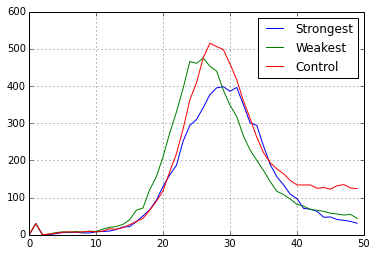
\includegraphics[max size={\textwidth}{\textheight}]{ADM Analysis_files/ADM Analysis_8_2.png}
    \par
    \end{center}
    
            \end{InvisibleVerbatim}
            
                \begin{InvisibleVerbatim}
                \vspace{-0.5\baselineskip}
    \begin{center}
    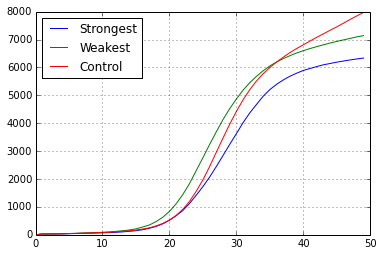
\includegraphics[max size={\textwidth}{\textheight}]{ADM Analysis_files/ADM Analysis_8_3.png}
    \par
    \end{center}
    
            \end{InvisibleVerbatim}
            
        
    


    % Make sure that atleast 4 lines are below the HR
    \needspace{4\baselineskip}

    
        \vspace{6pt}
        \makebox[0.1\linewidth]{\smaller\hfill\tt\color{nbframe-in-prompt}In\hspace{4pt}{[}712{]}:\hspace{4pt}}\\*
        \vspace{-2.65\baselineskip}
        \begin{ColorVerbatim}
            \vspace{-0.7\baselineskip}
            \begin{Verbatim}[commandchars=\\\{\}]
\PY{n}{pullExperiment}\PY{p}{(}\PY{l+s}{\PYZsq{}}\PY{l+s}{FtLewis6}\PY{l+s}{\PYZsq{}}\PY{p}{,}\PY{l+m+mi}{50}\PY{p}{)}
\end{Verbatim}

            
                \vspace{-0.2\baselineskip}
            
        \end{ColorVerbatim}
    

    

        % If the first block is an image, minipage the image.  Else
        % request a certain amount of space for the input text.
        \needspace{4\baselineskip}
        
        

            % Add document contents.
            
                \begin{InvisibleVerbatim}
                \vspace{-0.5\baselineskip}
\begin{alltt}<IPython.core.display.HTML at 0x111b411d0>\end{alltt}

            \end{InvisibleVerbatim}
            
                \begin{InvisibleVerbatim}
                \vspace{-0.5\baselineskip}
\begin{alltt}Experimental Variable v. Epistat Correlation coefficients:

Pharmaceutical Effectiveness
     attackRate   peakDay  peakNumber
ve    -0.025739 -0.025801   -0.047267
ate   -0.251619 -0.284967   -0.263670

Intervention Sequence
     attackRate       peakDay    peakNumber
vtd    0.058645 -2.310544e-02  7.469193e-02
atl    0.000000  7.661454e-19  9.222918e-18
apl    0.034913  3.311780e-02  5.445559e-02
sql   -0.016052 -4.659597e-02 -1.019704e-02


Attack Rate Extrema by Intervention Parameters

           Weakest Intervention Strongest Intervention
ve                           70                     30
vtd                          38                     17
ate                          87                     87
atl                          10                     10
apl                          10                     30
sq                           90                     90
sqg                          25                     25
sqtd                         10                     10
sql                           7                     28
other                 allonpost              allonpost
attackRate                 7164                   5398
peakDay                      27                     36
peakNumber                  461                    302
isEpidemic                   -1                     -1
leftBound                    17                     19
rightBound                   48                     50


Theoretical strongest and weakest pharmacuetical intervention (PI) \&
logistical implementation (LI):

Active Duty Military on base: 27663
Civilian Workers on post 15912

                Active Duty     Civilian Workers
Strong PI, Strong LI    24.607\%         0.044\%
Weak PI, Strong LI      24.159\%         0.013\%
Strong PI, Weak LI      24.444\%         0.019\%
Weak PI, Weak LI        24.166\%         0.038\%



\end{alltt}

            \end{InvisibleVerbatim}
            
                \begin{InvisibleVerbatim}
                \vspace{-0.5\baselineskip}
    \begin{center}
    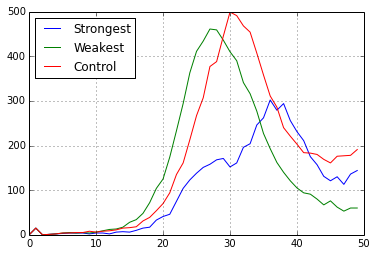
\includegraphics[max size={\textwidth}{\textheight}]{ADM Analysis_files/ADM Analysis_9_2.png}
    \par
    \end{center}
    
            \end{InvisibleVerbatim}
            
                \begin{InvisibleVerbatim}
                \vspace{-0.5\baselineskip}
    \begin{center}
    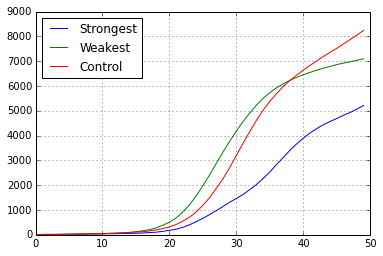
\includegraphics[max size={\textwidth}{\textheight}]{ADM Analysis_files/ADM Analysis_9_3.png}
    \par
    \end{center}
    
            \end{InvisibleVerbatim}
            
        
    


    % Make sure that atleast 4 lines are below the HR
    \needspace{4\baselineskip}

    
        \vspace{6pt}
        \makebox[0.1\linewidth]{\smaller\hfill\tt\color{nbframe-in-prompt}In\hspace{4pt}{[}713{]}:\hspace{4pt}}\\*
        \vspace{-2.65\baselineskip}
        \begin{ColorVerbatim}
            \vspace{-0.7\baselineskip}
            \begin{Verbatim}[commandchars=\\\{\}]
\PY{n}{pullExperiment}\PY{p}{(}\PY{l+s}{\PYZsq{}}\PY{l+s}{FtLewis7}\PY{l+s}{\PYZsq{}}\PY{p}{,}\PY{l+m+mi}{50}\PY{p}{)}
\end{Verbatim}

            
                \vspace{-0.2\baselineskip}
            
        \end{ColorVerbatim}
    

    

        % If the first block is an image, minipage the image.  Else
        % request a certain amount of space for the input text.
        \needspace{4\baselineskip}
        
        

            % Add document contents.
            
                \begin{InvisibleVerbatim}
                \vspace{-0.5\baselineskip}
\begin{alltt}<IPython.core.display.HTML at 0x112285510>\end{alltt}

            \end{InvisibleVerbatim}
            
                \begin{InvisibleVerbatim}
                \vspace{-0.5\baselineskip}
\begin{alltt}Experimental Variable v. Epistat Correlation coefficients:

Pharmaceutical Effectiveness
     attackRate   peakDay  peakNumber
ve    -0.075978 -0.075682   -0.093934
ate    0.200194  0.316148    0.227400

Intervention Sequence
     attackRate       peakDay    peakNumber
vtd   -0.017642 -4.734763e-02  3.631568e-02
atl    0.000000  2.543056e-18  8.127693e-18
apl   -0.010265 -3.802723e-02 -1.430956e-02
sql   -0.036417 -3.094373e-02 -2.554720e-02


Attack Rate Extrema by Intervention Parameters

           Weakest Intervention Strongest Intervention
ve                           70                     70
vtd                          38                     38
ate                          25                     87
atl                          10                     10
apl                          10                     10
sq                           90                     90
sqg                          25                     25
sqtd                         10                     10
sql                           7                     28
other                 allonpost                 active
attackRate                 7172                   5537
peakDay                      26                     27
peakNumber                  544                    270
isEpidemic                   -1                     -1
leftBound                    18                     17
rightBound                   47                     50


Theoretical strongest and weakest pharmacuetical intervention (PI) \&
logistical implementation (LI):

Active Duty Military on base: 27663
Civilian Workers on post 15912

                Active Duty     Civilian Workers
Strong PI, Strong LI    24.000\%         0.019\%
Weak PI, Strong LI      24.571\%         0.013\%
Strong PI, Weak LI      24.079\%         0.031\%
Weak PI, Weak LI        24.632\%         0.031\%



\end{alltt}

            \end{InvisibleVerbatim}
            
                \begin{InvisibleVerbatim}
                \vspace{-0.5\baselineskip}
    \begin{center}
    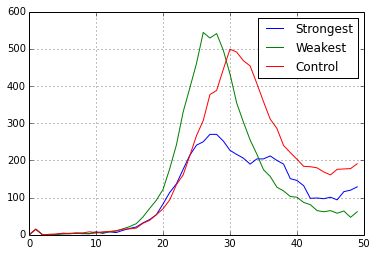
\includegraphics[max size={\textwidth}{\textheight}]{ADM Analysis_files/ADM Analysis_10_2.png}
    \par
    \end{center}
    
            \end{InvisibleVerbatim}
            
                \begin{InvisibleVerbatim}
                \vspace{-0.5\baselineskip}
    \begin{center}
    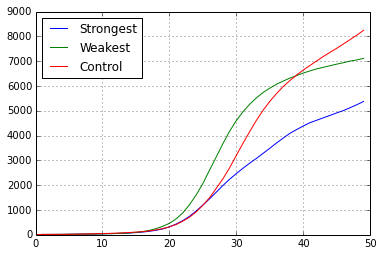
\includegraphics[max size={\textwidth}{\textheight}]{ADM Analysis_files/ADM Analysis_10_3.png}
    \par
    \end{center}
    
            \end{InvisibleVerbatim}
            
        
    


    % Make sure that atleast 4 lines are below the HR
    \needspace{4\baselineskip}

    
        \vspace{6pt}
        \makebox[0.1\linewidth]{\smaller\hfill\tt\color{nbframe-in-prompt}In\hspace{4pt}{[}714{]}:\hspace{4pt}}\\*
        \vspace{-2.65\baselineskip}
        \begin{ColorVerbatim}
            \vspace{-0.7\baselineskip}
            \begin{Verbatim}[commandchars=\\\{\}]
\PY{n}{pullExperiment}\PY{p}{(}\PY{l+s}{\PYZsq{}}\PY{l+s}{FtLewis8}\PY{l+s}{\PYZsq{}}\PY{p}{,}\PY{l+m+mi}{50}\PY{p}{)}
\end{Verbatim}

            
                \vspace{-0.2\baselineskip}
            
        \end{ColorVerbatim}
    

    

        % If the first block is an image, minipage the image.  Else
        % request a certain amount of space for the input text.
        \needspace{4\baselineskip}
        
        

            % Add document contents.
            
                \begin{InvisibleVerbatim}
                \vspace{-0.5\baselineskip}
\begin{alltt}<IPython.core.display.HTML at 0x111b41f50>\end{alltt}

            \end{InvisibleVerbatim}
            
                \begin{InvisibleVerbatim}
                \vspace{-0.5\baselineskip}
\begin{alltt}Experimental Variable v. Epistat Correlation coefficients:

Pharmaceutical Effectiveness
     attackRate   peakDay  peakNumber
ve    -0.006836 -0.028484   -0.029189
ate   -0.274242 -0.266242   -0.269018

Intervention Sequence
       attackRate       peakDay    peakNumber
vtd  5.587836e-03 -1.032527e-01  4.553079e-02
atl -6.646898e-18 -2.698500e-18  1.150571e-17
apl -1.055713e-02 -3.956043e-03 -4.027322e-03
sql  2.674206e-02  2.373626e-03  2.466300e-02


Attack Rate Extrema by Intervention Parameters

           Weakest Intervention Strongest Intervention
ve                           70                     30
vtd                          38                     17
ate                          87                     87
atl                          10                     10
apl                          10                     10
sq                           90                     90
sqg                          25                     25
sqtd                         10                     10
sql                           7                      7
other                 allonpost                 active
attackRate                 7094                   5831
peakDay                      27                     30
peakNumber                  534                    261
isEpidemic                   -1                     -1
leftBound                    17                     19
rightBound                   47                     50


Theoretical strongest and weakest pharmacuetical intervention (PI) \&
logistical implementation (LI):

Active Duty Military on base: 27663
Civilian Workers on post 15912

                Active Duty     Civilian Workers
Strong PI, Strong LI    24.621\%         0.031\%
Weak PI, Strong LI      24.028\%         0.063\%
Strong PI, Weak LI      23.826\%         0.013\%
Weak PI, Weak LI        24.141\%         0.050\%



\end{alltt}

            \end{InvisibleVerbatim}
            
                \begin{InvisibleVerbatim}
                \vspace{-0.5\baselineskip}
    \begin{center}
    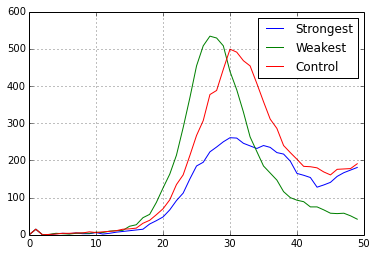
\includegraphics[max size={\textwidth}{\textheight}]{ADM Analysis_files/ADM Analysis_11_2.png}
    \par
    \end{center}
    
            \end{InvisibleVerbatim}
            
                \begin{InvisibleVerbatim}
                \vspace{-0.5\baselineskip}
    \begin{center}
    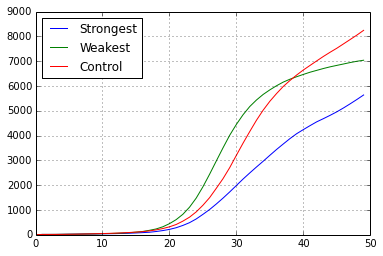
\includegraphics[max size={\textwidth}{\textheight}]{ADM Analysis_files/ADM Analysis_11_3.png}
    \par
    \end{center}
    
            \end{InvisibleVerbatim}
            
        
    


    % Make sure that atleast 4 lines are below the HR
    \needspace{4\baselineskip}

    
        \vspace{6pt}
        \makebox[0.1\linewidth]{\smaller\hfill\tt\color{nbframe-in-prompt}In\hspace{4pt}{[}715{]}:\hspace{4pt}}\\*
        \vspace{-2.65\baselineskip}
        \begin{ColorVerbatim}
            \vspace{-0.7\baselineskip}
            \begin{Verbatim}[commandchars=\\\{\}]
\PY{n}{pullExperiment}\PY{p}{(}\PY{l+s}{\PYZsq{}}\PY{l+s}{FtLewis9}\PY{l+s}{\PYZsq{}}\PY{p}{,}\PY{l+m+mi}{50}\PY{p}{)}
\end{Verbatim}

            
                \vspace{-0.2\baselineskip}
            
        \end{ColorVerbatim}
    

    

        % If the first block is an image, minipage the image.  Else
        % request a certain amount of space for the input text.
        \needspace{4\baselineskip}
        
        

            % Add document contents.
            
                \begin{InvisibleVerbatim}
                \vspace{-0.5\baselineskip}
\begin{alltt}<IPython.core.display.HTML at 0x112285550>\end{alltt}

            \end{InvisibleVerbatim}
            
                \begin{InvisibleVerbatim}
                \vspace{-0.5\baselineskip}
\begin{alltt}Experimental Variable v. Epistat Correlation coefficients:

Pharmaceutical Effectiveness
     attackRate   peakDay  peakNumber
ve    -0.073782  0.008363   -0.064721
ate   -0.261181 -0.348168   -0.280434

Intervention Sequence
       attackRate   peakDay    peakNumber
vtd  8.023694e-02 -0.020600  1.136680e-01
atl  4.861192e-18  0.000000  6.784788e-18
apl -2.953274e-02 -0.051195 -2.939462e-02
sql -2.038740e-02 -0.031207 -1.055222e-02


Attack Rate Extrema by Intervention Parameters

           Weakest Intervention Strongest Intervention
ve                           30                     70
vtd                          38                     17
ate                          87                     87
atl                          10                     10
apl                          10                     10
sq                           90                     90
sqg                          25                     25
sqtd                         10                     10
sql                           7                      7
other                 allonpost              allonpost
attackRate                 7144                   5547
peakDay                      26                     27
peakNumber                  489                    432
isEpidemic                   -1                     -1
leftBound                    18                     17
rightBound                   47                     49


Theoretical strongest and weakest pharmacuetical intervention (PI) \&
logistical implementation (LI):

Active Duty Military on base: 27663
Civilian Workers on post 15912

                Active Duty     Civilian Workers
Strong PI, Strong LI    24.560\%         0.019\%
Weak PI, Strong LI      24.173\%         0.057\%
Strong PI, Weak LI      23.045\%         0.214\%
Weak PI, Weak LI        24.600\%         0.101\%



\end{alltt}

            \end{InvisibleVerbatim}
            
                \begin{InvisibleVerbatim}
                \vspace{-0.5\baselineskip}
    \begin{center}
    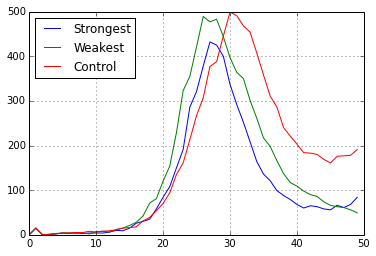
\includegraphics[max size={\textwidth}{\textheight}]{ADM Analysis_files/ADM Analysis_12_2.png}
    \par
    \end{center}
    
            \end{InvisibleVerbatim}
            
                \begin{InvisibleVerbatim}
                \vspace{-0.5\baselineskip}
    \begin{center}
    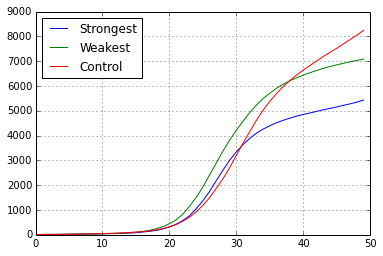
\includegraphics[max size={\textwidth}{\textheight}]{ADM Analysis_files/ADM Analysis_12_3.png}
    \par
    \end{center}
    
            \end{InvisibleVerbatim}
            
        
    


    % Make sure that atleast 4 lines are below the HR
    \needspace{4\baselineskip}

    
        \vspace{6pt}
        \makebox[0.1\linewidth]{\smaller\hfill\tt\color{nbframe-in-prompt}In\hspace{4pt}{[}715{]}:\hspace{4pt}}\\*
        \vspace{-2.65\baselineskip}
        \begin{ColorVerbatim}
            \vspace{-0.7\baselineskip}
            \begin{Verbatim}[commandchars=\\\{\}]

\end{Verbatim}

            
                \vspace{0.3\baselineskip}
            
        \end{ColorVerbatim}
    

        

        \renewcommand{\indexname}{Index}
        \printindex

    % End of document
    \end{document}


